\documentclass[a4paper,12pt]{report}
\usepackage[utf8]{inputenc}
\usepackage[T1]{fontenc}
\usepackage[french]{babel} 
\usepackage{xcolor,graphicx}
\usepackage{enumitem}
\usepackage{hyperref}
\usepackage[margin=0in]{geometry}
\graphicspath{{image/}}
\usepackage{graphicx}

\begin{document}


\underline{\textbf{LES DIFFERENTS CAPTEURS}}


\hfill

\begin{itemize} 
\setlength{\itemindent}{1cm}
 \item \underline{\textbf{BMP180:}}
\end{itemize}

\setlength{\itemindent}{3cm}

Le BMP180 est composé principalement d'un \underline{capteur piézo-résistif},d'un \underline{convertisseur analogique vers digital} 
et \\ une \underline{unité de contrôle composé d'un EEPROM et de l'interface I2C série}.\\

Ce capteur est designé pour être \textbf{directement connecté au microcontrôlleur} grâce au bus I2C. 

\begin{itemize}
\centering
\setlength{\itemindent}{2cm}
\item \underline{\textit{\textbf{Principe de fonctionnement:}}} Comme le capteur à une "unité de
 contrôle" elle lui permet de mesurer la pression après un laps de temps donné et d'avoir le résultat des calculs.    
\end{itemize} 


\centering
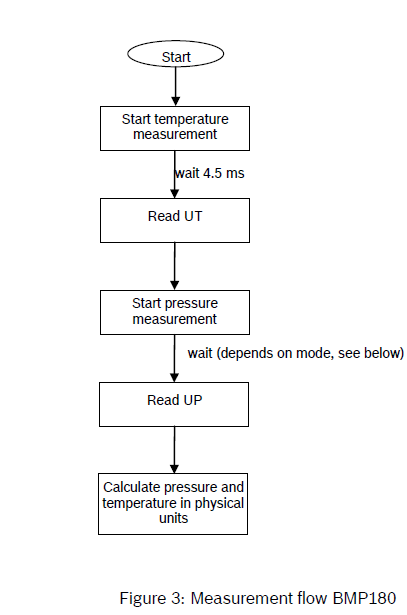
\includegraphics[width=0.35\textwidth]{2.png}



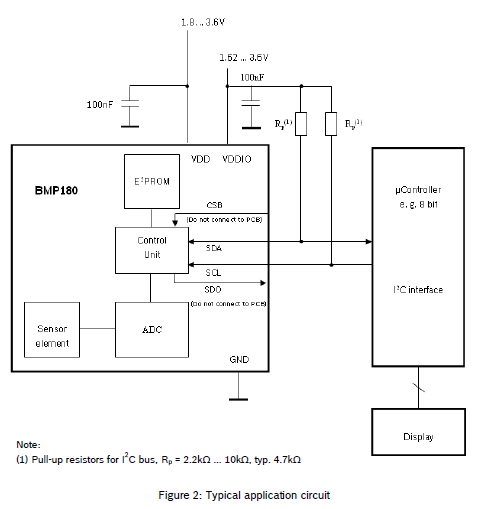
\includegraphics[width=0.50\textwidth]{sblck.png}\\

\vspace{3cm}
\hfill

\begin{itemize}
\vspace{2cm}
\setlength{\itemindent}{2cm}
\item \underline{\textit{\textbf{Plage de valeurs mesurée:}}} L'intervalle est de \textbf{300} à \textbf{1100hPa} (110.000 Pa)
\end{itemize} 

\begin{itemize}
\setlength{\itemindent}{2cm}
\item \underline{\textit{\textbf{Tension d'alimentation:}}} Entre \textbf{1.8} à \textbf{3.6V} 
\end{itemize} 

\vspace{1cm}

\begin{itemize} 
\setlength{\itemindent}{1cm}
 \item \underline{\textbf{MPX4115A:}}
\end{itemize}




\end{document}
